%document class
\documentclass{article}


%package
\usepackage{ctex}      % 中文支持
\usepackage{amsmath}   % Advanced math typesetting
\usepackage{amsfonts}
\usepackage{hyperref}  % Add a link to your document
\usepackage{graphicx}  % Add pictures to your document
\usepackage{subcaption}% Add sub figure support
\usepackage{listings}  % Source code formatting and highlighting
\usepackage[backend=bibtex]{biblatex} % Use biblatex package
%\bibliography{cite}	    % Cite database name

% page setting
\usepackage{geometry}
\geometry{left=2.5cm, right=2.5cm, top=2.0cm, bottom=2.0cm}

%document body
\begin{document}

%============================================
\title{Berkeley CS285 Notes}
\author{}
\date{}
\maketitle{}          % Generate title


%contents 目录
\renewcommand{\contentsname}{\centering Contents}
\tableofcontents{}    % Generate contents


\newpage{}
\section{Deep Reinforcement Learning, Decision Making, and Control}


%============================================
\subsection{What is reinforcement learning, and why should we care?}
How do we build intelligent machines?

Intelligent machines must be able to adapt

Deep learning helps us handle unstructured environments

Reinforcement learning provides a formalism for behavior
\begin{figure}[h!] % Here
	\centering
	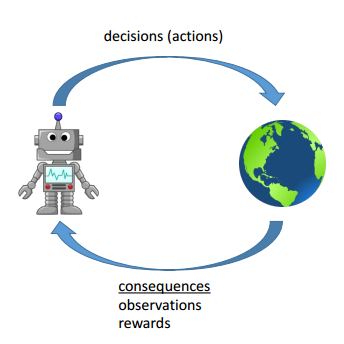
\includegraphics[width=0.5\linewidth]{img/1-formalism.png}
	\caption{a formalism for behavior}\label{img:1-formalism}
\end{figure}


What is deep RL, and why should we care?
\begin{figure}[h!] % Here
	\centering
	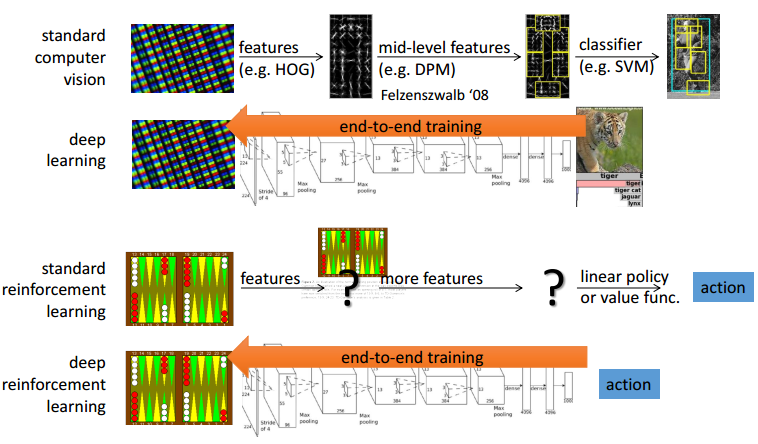
\includegraphics[width=0.8\linewidth]{img/1-end-to-end.png}
	\caption{end to end loop}\label{img:1-end-to-end}
\end{figure}


%============================================
\subsection{What does end-to-end learning mean for sequential decision making?}
perception (tiger) -> action (run away). 

sensorimotor loop.

Example: robotics
\begin{figure}[h!] % Here
	\centering
	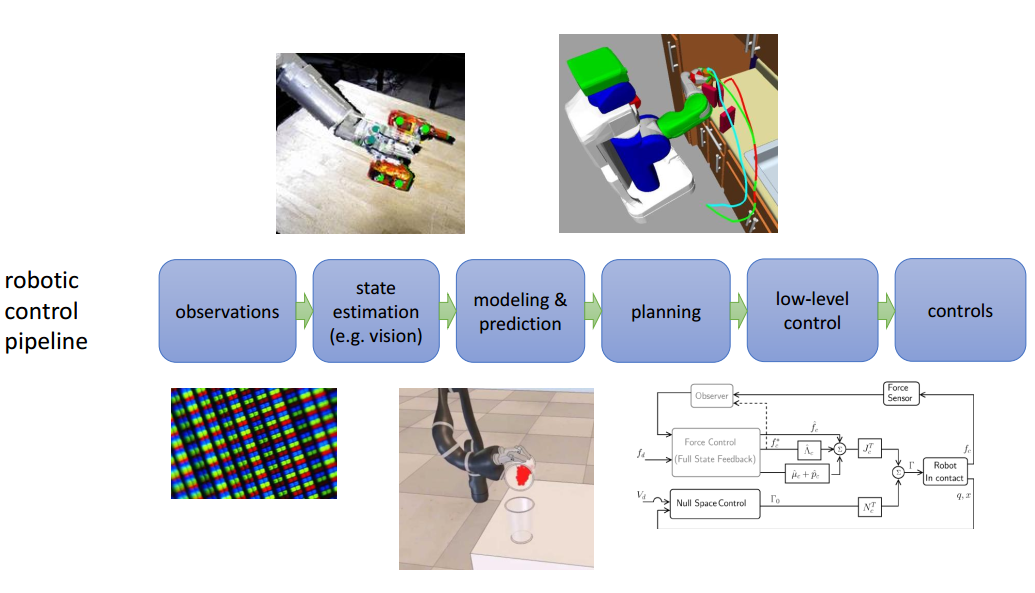
\includegraphics[width=0.8\linewidth]{img/1-robotics.png}
	\caption{robotics}\label{img:1-robotics}
\end{figure}

Deep models are what allow reinforcement
learning algorithms to solve complex problems
end to end!

The reinforcement learning problem is the AI problem!

Why should we study this now?
\begin{itemize}
	\item Advances in deep learning
	\item Advances in reinforcement learning
	\item Advances in computational capability
\end{itemize}


%============================================
\subsection{What other problems do we need to solve to 
enable real-world sequential decision making?}

\subsubsection{Beyond learning from reward}
\begin{itemize}
	\item Basic reinforcement learning deals with maximizing rewards
	\item This is not the only problem that matters for sequential decision
	making!
	\item We will cover more advanced topics
		\begin{itemize}
			\item Learning reward functions from example (inverse reinforcement learning)
			\item Transferring knowledge between domains (transfer learning, meta-learning)
			\item Learning to predict and using prediction to act
		\end{itemize}
\end{itemize}

\subsubsection{Where do rewards come from?}
Game scores.

Animals as food for tiger.


\subsubsection{Are there other forms of supervision?}
\begin{itemize}
	\item Learning from demonstrations
		\begin{itemize}
			\item Directly copying observed behavior 
			\item Inferring rewards from observed behavior (inverse reinforcement learning) 
		\end{itemize}
	\item Learning from observing the world
		\begin{itemize}
			\item Learning to predict 
			\item Unsupervised learning 
		\end{itemize}
	\item Learning from other tasks 
		\begin{itemize}
			\item Transfer learning 
			\item Meta-learning: learning to learn
		\end{itemize}
\end{itemize}


%============================================
\subsection{How do we build intelligent machines?}
Imagine you have to build an intelligent machine, where do you start?

\subsubsection{Learning as the basis of intelligence}
Some things we can all do (e.g. walking).
Some things we can only learn (e.g. driving a car).
We can learn a huge variety of things, including very difficult things.
Therefore our learning mechanism(s) are likely powerful enough to do
everything we associate with intelligence.

\subsubsection{A single algorithm?}
An algorithm for each “module”?

Or a single flexible algorithm?

\subsubsection{What must that single algorithm do?}
Interpret rich sensory inputs

Choose complex actions

\subsubsection{Why deep reinforcement learning?}
Deep = can process complex sensory input... and also compute really complex functions

Reinforcement learning = can choose complex actions.


\subsubsection{What has proven challenging so far?}
Humans can learn incredibly quickly, Deep RL methods are usually slow

Humans can reuse past knowledge, Transfer learning in deep RL is an open problem

Not clear what the reward function should be

Not clear what the role of prediction should be


What is deep RL, and why should we care?
\begin{figure}[h!] % Here
	\centering
	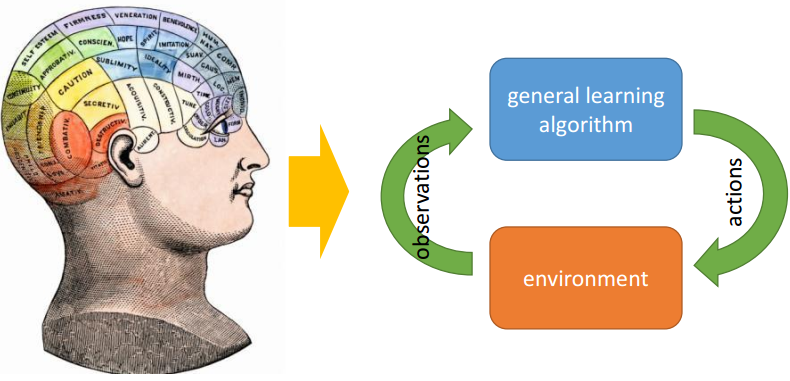
\includegraphics[width=0.5\linewidth]{img/1-human.png}
	\caption{child}\label{img:1-human}
\end{figure}

Instead of trying to produce a
program to simulate the adult
mind, why not rather try to
produce one which simulates the
child's? If this were then subjected
to an appropriate course of
education one would obtain the
adult brain. --Alan Turing








%bibliography
\newpage{}
\printbibliography

%============================================
\end{document}